\documentclass{article}
%%% INICIO DEL PREÁMBULO %%%

\usepackage[greek,spanish,es-tabla,es-nodecimaldot,es-noindentfirst]{babel}
\usepackage{fontspec}
\setmonofont{Consolas Bold}
\usepackage{babelbib}
\usepackage{nccmath}
\usepackage[oldvoltagedirection]{circuitikz}
\usepackage{amsthm}
\usepackage{lipsum}
\usepackage{tcolorbox}
\usepackage[thicklines]{cancel}
\usepackage{mathtools}
\usepackage{amssymb}
\usepackage{amsmath}
\usepackage[listformat=empty]{caption}
\captionsetup{
         listformat=empty,
         justification=justified,
		 font=Large
}
\usepackage[titles]{tocloft}
\cftsetindents{figure}{0em}{1.5em}
\renewcommand{\cftdot}{}

\usepackage{subcaption}   
\usepackage{color}       
\usepackage{verbatim}     
\usepackage{enumerate}
\usepackage{geometry} 
\geometry{a4paper,left=35mm,right=35mm,top=15mm,bottom=15mm}
\usepackage{isotope}
\usepackage{maybemath} 
\usepackage{upgreek}
\usepackage{wasysym} 
\usepackage[italic]{hepparticles}
\usepackage{subdepth}
\usepackage[italicdiff]{physics}
\usepackage{braket}
\usepackage{tensor}
\usepackage{chemformula} 
\usepackage{tikz} \usetikzlibrary{babel}
\usepackage{siunitx}
\usepackage{url}
\usepackage{listings}
\usepackage{multirow}
\usepackage{multicol}
\usepackage[colorlinks=true]{hyperref}
\hypersetup{
citecolor = blue,
linkcolor = blue,
urlcolor = blue,
pdfauthor = {Javier Rodrigo López}
}
\usepackage{eso-pic}
\usepackage{siunitx}
\sisetup{
round-mode      = places,
round-precision = 2,
}

% tikz
\usepackage{tikz} \usetikzlibrary{fit,babel,shapes,arrows,positioning}
\tikzstyle{block} = [draw, fill=white, rectangle, 
    minimum height=3em, minimum width=6em]
\tikzstyle{sum} = [draw, fill=white, circle, node distance=1cm]
\tikzstyle{input} = [coordinate]
\tikzstyle{output} = [coordinate]
\tikzstyle{pinstyle} = [pin edge={to-,thin,black}]
\tikzset{
block/.style = {draw, fill=white, rectangle, minimum height=3em, minimum width=3em},
tmp/.style  = {coordinate}, 
sum/.style= {draw, fill=white, circle, node distance=1cm},
input/.style = {coordinate},
output/.style= {coordinate},
pinstyle/.style = {pin edge={to-,thin,black}}
}

% Títulos
\usepackage{titlesec}
\titleformat{\section}
	{\normalfont\Large\bfseries}{\thesection}{1em}{}[{\titlerule[0.8pt]}]
\titleformat{\subsubsection}
	{\normalfont\normalsize\bfseries}{\thesubsubsection}{1em}{}[{\titlerule[0.05pt]}]
\titlespacing{\section}{0pt}{2\parskip}{\parskip}
\titlespacing{\subsection}{0pt}{\parskip}{0pt}
\titlespacing{\subsubsection}{0pt}{\parskip}{0pt}

% Numeración de secciones
\setcounter{tocdepth}{2}
\setcounter{secnumdepth}{2}

% Enumerations
\newcounter{myenumi}
\renewcommand{\themyenumi}{\alph{myenumi})}
\newenvironment{myenumerate}{\setlength{\parindent}{0pt}\setcounter{myenumi}{0}\renewcommand{\item}{\par\refstepcounter{myenumi}\makebox[1.3em][l]{\themyenumi}}}{\par\bigskip\noindent\ignorespacesafterend}

% Organización del texto
\newcommand{\formula}[1]{\vspace{13 pt}\noindent \textbf{\underline{#1}}}
\newcommand{\subtext}[1]{_{\text{#1}}}

% Unidades y utilidades varias
\renewcommand{\S}{\operatorname{S}}
\newcommand{\dB}{\operatorname{dB}}
\newcommand{\dBW}{\operatorname{dBW}}
\newcommand{\dBm}{\operatorname{dBm}}
\newcommand{\Hz}{\operatorname{Hz}}
\newcommand{\s}{\operatorname{s}}
\newcommand{\A}{\operatorname{A}}
\newcommand{\V}{\operatorname{V}}
\newcommand{\ohm}{\,\Omega}
\newcommand{\Pa}{\operatorname{Pa}}
\newcommand{\W}{\operatorname{W}}
\newcommand{\I}{\operatorname{I}}
\newcommand{\K}{\operatorname{K}}
\newcommand{\m}{\operatorname{m}}
\newcommand{\mm}{\operatorname{mm}}
\newcommand{\rad}{\operatorname{rad}}
\newcommand{\mol}{\operatorname{mol}}
\newcommand{\J}{\operatorname{J}}
\newcommand{\kg}{\operatorname{kg}}
\newcommand{\incremento}{\Delta}
\newcommand{\psus}{\, \ldots \,}
\newcommand{\sen}{\operatorname{\sen}}
\renewcommand{\sin}{\sen}
\renewcommand{\arcsin}{\arcsen}
\renewcommand{\arctan}{\arctg}
\renewcommand{\min}{\operatorname{mín}}

\definecolor{mygreen}{RGB}{28,172,0} % color values Red, Green, Blue
\definecolor{mylilas}{RGB}{170,55,241}

\lstset{language=Matlab,
	numbers=none,
    breaklines=true,
    morekeywords={matlab2tikz},
    keywordstyle=\color{blue},
    morekeywords=[2]{1}, keywordstyle=[2]{\color{black}},
    identifierstyle=\color{black},
    stringstyle=\color{mylilas},
    commentstyle=\color{mygreen},
	showspaces=false,
    showstringspaces=false,
    numberstyle={\tiny \color{black}},
    numbersep=9pt,
    emph=[1]{for,end,break},emphstyle=[1]\color{red},
	escapeinside={\%*}{*)},
	basicstyle=\footnotesize\ttfamily,
	columns=flexible
}

% Vectores
\usepackage[c]{esvect}
\renewcommand{\vec}[1]{\vv{{#1}}}
\newcommand{\proy}[2]{\operatorname{proy}_{\vec{#2}}\vec{#1}}
\newcommand{\antiparallel}{\downharpoonleft \! \upharpoonright}
\newcommand{\parallelvec}{\upharpoonleft \! \upharpoonright}

% Espaciado
\usepackage{enumitem}
\setlist{before={\parskip=3pt}, after=\vspace{\baselineskip}}
\setlength{\parindent}{0pt}
\setlength{\parskip}{0.5em}

% Estadística
\DeclareMathOperator{\Var}{Var}
\DeclareMathOperator{\Cov}{Cov}
\renewcommand{\var}{\sigma ^2}
\DeclareMathOperator{\B}{B}
\DeclareMathOperator{\BN}{BN}
\DeclareMathOperator{\Geo}{Geo}
\DeclareMathOperator{\Poisson}{Poisson}
\DeclareMathOperator{\Exp}{Exp}
\DeclareMathOperator{\N}{N}
\DeclareMathOperator{\Mult}{Mult}
\newcommand{\probCond}[2]{P \left( #1 \: \middle\vert\:  #2 \right) }

% Electromagnetismo y Ondas
\newcommand{\errorGrave}{\textbf{FG!!!}}
\newcommand{\mas}{M.A.S.}
\newcommand{\mcu}{M.C.U.}
\newcommand{\ed}{E.D.}
\newcommand{\edmas}{E.D. del M.A.S.}
\usepackage{esint}

% Señales y Sistemas
\renewcommand{\H}{H}

% Circled number
\newcommand{\circledNumber}[1]{\raisebox{.9pt}{\textcircled{\raisebox{-.9pt}{#1}}}}

% Footnotes
% \renewcommand{\thefootnote}{\fnsymbol{footnote}}

%%% FIN DEL PREÁMBULO %%%

% Título y portada
\title{\Huge Informe Práctica 1\\\vspace*{5pt}
\Large Señales y Sistenas}
\author{Javier Rodrigo López \thanks{Correo electrónico: \href{mailto:javier.rlopez@alumnos.upm.es}{\texttt{javier.rlopez@alumnos.upm.es}}}} 
\date{\today}

%%% INICIO DEL DOCUMENTO %%%
\begin{document}

\maketitle

\tableofcontents
\setlength{\cftparskip}{0.5\baselineskip}
\listoffigures

\newpage

\section{Introducción}
Las figuras que se adjuntan aparecen en el mismo orden en el cual son generadas al ejecutar el script de MATLAB.

Por lo tanto, se debe mirar el código para entender qué gráfica se genera en cada apartado y a qué ejercicio corresponde.

\newpage

\section{Código}
\pagestyle{empty}
\begin{lstlisting}
% Autor: Javier Rodrigo López
% Laboratorio de Señales y Sistemas - Práctica 1
% Fecha de finalización: 02/03/2021
%
% Para visualizar esta práctica, se ha implementado la función 'pause', por
% lo que durante la ejecución cada gráfica se generará al pulsar la tecla
% Enter. La última vez que sea pulsada, cerrará todas las ventanas.

%% Preámbulo
% Comandos útiles
clear all
clc
close all

% Definición de señales impulso y escalón
d = @(t) t == 0;
u = @(t) t >= 0;

% Constantes
n1 = 10;
N1 = 15;
n2 = 8;
n3 = 11;
z0 = (5/4) * exp(1i * pi / 6);
n4 = 4;
n5 = 8;
X0 = -2;
X1 = 4;
t0 = -4;
t1 = 8;
T1 = 10;
s0 = 2 + 8 * pi * 1i;
t2 = 4;
T2 = -6;
T3 = 8;
alfa1 = 1/2;
alfa2 = 5;
step = 1E-3;

%% Ejercicio 1
n = -N1:N1;

x1 = @(n) n.^2 .* (u(n) - u(n - n1));
x2 = @(n) cos(pi * n / 2) .* (u(n + n3) - u(n - n2));
x3 = @(n) z0.^n .* (u(n + n4) .* u(-n + n5));

figure
stem(n, x1(n)), title('Señal x_1[n]'), xlabel('n'), ylabel('Amplitud');
pause

figure
stem(n, x2(n)), title('Señal x_2[n]'), xlabel('n'), ylabel('Amplitud');
pause

figure
subplot(2, 1, 1)
stem(n, real(x3(n))), title('Señal x_3[n]'), xlabel('n'), ylabel('Parte real');
subplot(2, 1, 2)
stem(n, imag(x3(n))), xlabel('n'), ylabel('Parte imaginaria');
pause

figure
subplot(2, 1, 1)
stem(n, abs(x3(n))), title('Señal x_3[n]'), xlabel('n'), ylabel('Módulo');
subplot(2, 1, 2)
stem(n, angle(x3(n))), xlabel('n'), ylabel('Fase');
pause
%% Ejercicio 2
t = T2:step:T3;

x1c = exp(-s0 .* t) .* (u(t + t2) - u(t - t2)); % La c indica que es continua.

figure
subplot(2, 1, 1)
plot(t, real(x1c)), title('Señal x_1(t)'), xlabel('t'), ylabel('Parte real');
subplot(2, 1, 2)
plot(t, imag(x1c)), xlabel('t'), ylabel('Parte imaginaria');
pause

t = -T1:step:T1;

x2c = (t0 <= t & t < X0) * 4 .* cos(X0 * t / 4) + (X0 <= t & t < X1 - X0) .* t.^2 + (X1 - X0 <= t & t <= t1) .* (-t + X0);

figure
plot(t, x2c), title('Señal x_2(t)'), xlabel('t'), ylabel('Amplitud');
pause

%% Ejercicio 3
% La variable 'n' ya fue definido en el primer ejercicio.

x7 = alfa1 * x1(n) + alfa2 * x2(n);
x8 = x1(n) .* x2(n);
x9 = conj(x3(n));

figure
stem(n, x7), title('Señal x_7[n]'), xlabel('n'), ylabel('Amplitud');
pause

figure
stem(n, x8), title('Señal x_8[n]'), xlabel('n'), ylabel('Amplitud');
pause

figure
subplot(2, 1, 1)
stem(n, real(x9)), title('Señal x_9[n]'), xlabel('n'), ylabel('Parte real');
subplot(2, 1, 2)
stem(n, imag(x9)), xlabel('n'), ylabel('Parte imaginaria');
pause

%% Ejercicio 4

x1p = (x1(n) + x1(-n)) / 2;
x1i = (x1(n) - x1(-n)) / 2;

figure
subplot(2, 1, 1)
stem(n, x1p), title('Parte par de x_1[n]'), xlabel('n'), ylabel('Amplitud');
subplot(2, 1, 2)
stem(n, x1i), title('Parte impar de x_1[n]'), xlabel('n'), ylabel('Amplitud');
pause

close all
\end{lstlisting}

\newpage
\pagestyle{plain} 
\section{Figuras}

\begin{figure}[h] \caption[Figura 1]{}
	\centering
		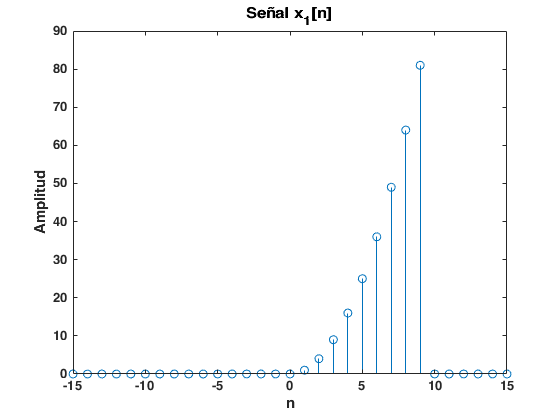
\includegraphics[width=\linewidth]{./Figures/01.png}
\end{figure}

\begin{figure}[h!] \caption[Figura 2]{}
	\centering
		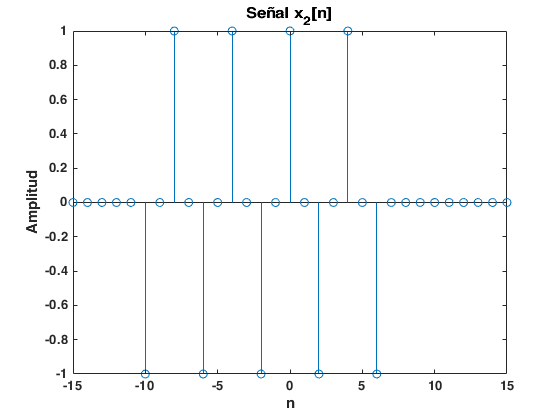
\includegraphics[width=\linewidth]{./Figures/02.png}
\end{figure}

\begin{figure} \caption[Figura 3]{}
	\centering
		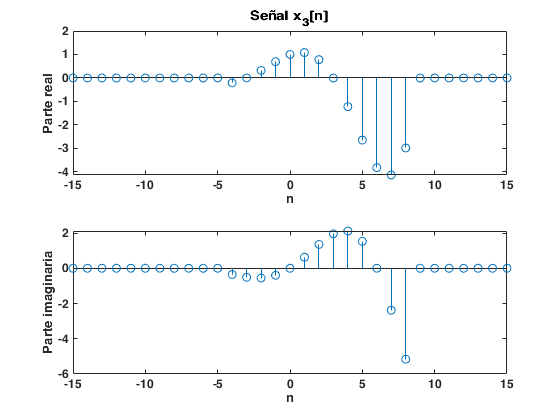
\includegraphics[width=\linewidth]{./Figures/03.png}
\end{figure}

\begin{figure} \caption[Figura 4]{}
	\centering
		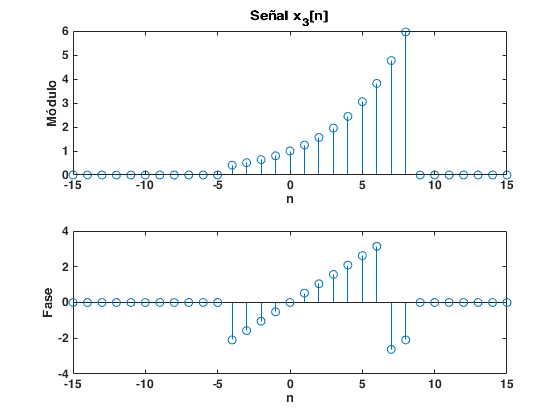
\includegraphics[width=\linewidth]{./Figures/04.png}
\end{figure}

\begin{figure} \caption[Figura 5]{}
	\centering
		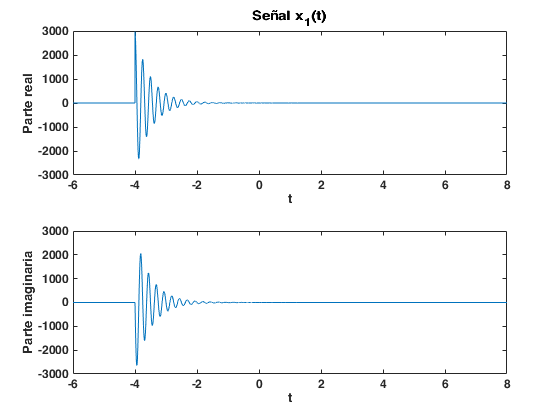
\includegraphics[width=\linewidth]{./Figures/05.png}
\end{figure}

\begin{figure} \caption[Figura 6]{}
	\centering
		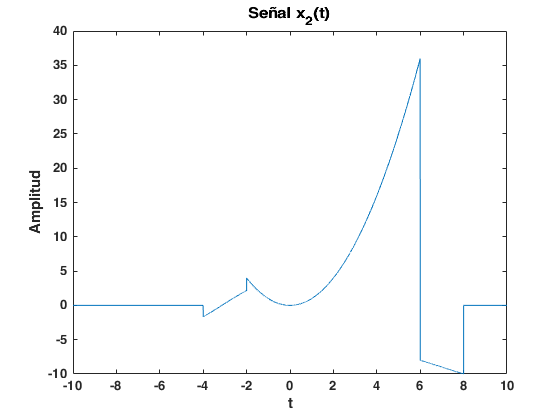
\includegraphics[width=\linewidth]{./Figures/06.png}
\end{figure}

\begin{figure} \caption[Figura 7]{}
	\centering
		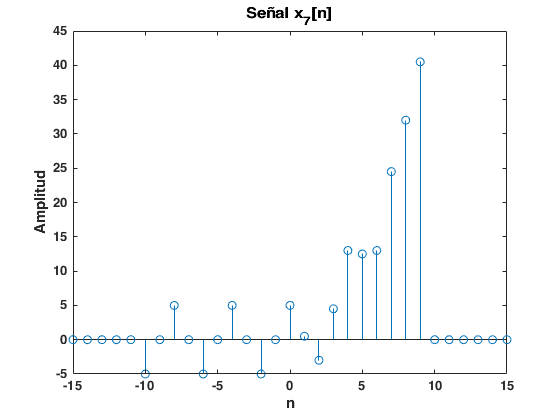
\includegraphics[width=\linewidth]{./Figures/07.png}
\end{figure}

\begin{figure} \caption[Figura 8]{}
	\centering
		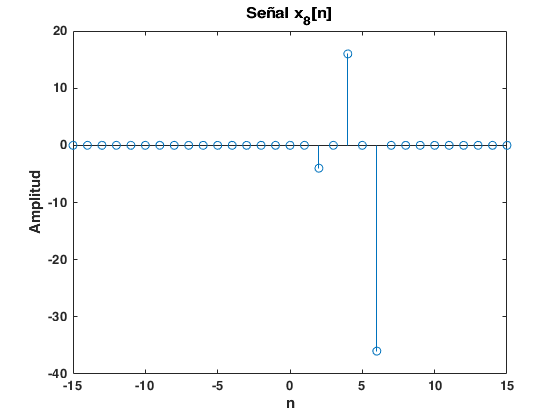
\includegraphics[width=\linewidth]{./Figures/08.png}
\end{figure}

\begin{figure} \caption[Figura 9]{}
	\centering
		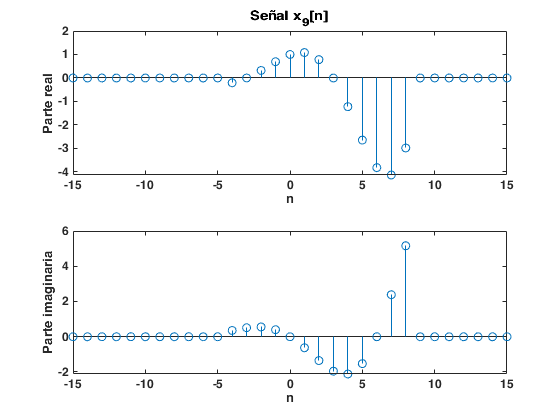
\includegraphics[width=\linewidth]{./Figures/09.png}
\end{figure}

\begin{figure} \caption[Figura 10]{}
	\centering
		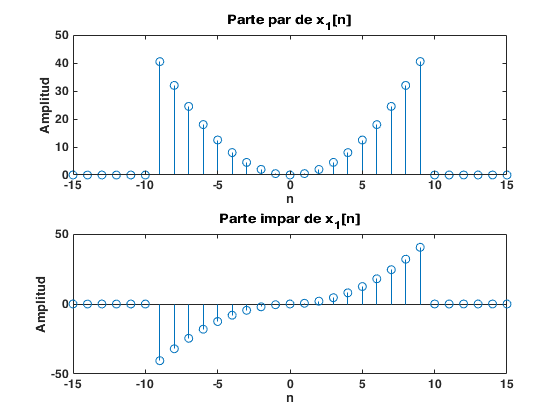
\includegraphics[width=\linewidth]{./Figures/10.png}
\end{figure}

\end{document}